% !TeX root = ../diss.tex
\chapter{Implementation}
\textit{In this chapter I describe how my PPL is implemented and the design decisions considered. I discuss the core data structures used to represent distributions and how inference was implemented over these. I also describe auxiliary functionality included, such as visualisation functions. Finally, I describe the challenges of testing a probabilistic system and how I overcame them. Documentation for all publicly exposed functions can be found in appendix \ref{app:docs}.}

\section{Repository Overview}

\begin{wrapfigure}[25]{R}{0.4\textwidth}
	\dirtree{%
		.1 ppl.
		% .2 \_build.
		% .2 \_coverage.
		.2 bin.
		.3 \dots.
		.2 doc.
		.3 \dots.
		.2 lib.
		.3 inference.
		.4 \dots.
		.3 dist.ml.
		.3 empirical.ml.
		.3 helpers.ml.
		.3 inference.ml.
		.3 monad.ml.
		.3 plot.ml.
		.3 ppl.ml.
		.3 primitive.ml.
		.2 test.
		.3 unit\_tests.
		.4 \dots.
		.3 test\_models.ml.
		.3 hypothesis\_tests.ml.
		.2 dune-project.
		.2 ppl.opam.
	}
	\caption{Directory structure}
	\label{fig:dirs}
\end{wrapfigure}

The code for the PPL library is in the \texttt{ppl} directory, which contains the core library, unit tests, statistical testing code and some example programs written using the library. A separate evaluation folder contains code to benchmark my PPL's performance compared to other languages.

The structure follows the de facto standard for dune projects. The lib directory contains all the code for the library, bin contains standalone scripts which contain example models, doc contains auto-generated documentation, and test contains unit and hypothesis tests. The ppl.opam file describes my library and it's dependencies, to allow my library to be distributed via opam.

The lib directory contains several modules to separate functionality within my PPL. The entry point is the Ppl module, which exports the other modules so that opening Ppl is sufficient to define models. The inference directory contains inference algorithms in separate modules, which are then re-exported in the main Inference module. The Dist module is the module for user-defined models on which inference is run. 

All code is written in OCaml 4.08, with the main dependencies being Jane Street's \texttt{Core} and \texttt{Owl} \cite{owl}.	
	
\section{Language Design}
% specify DSL here 
I chose to implement my language as a domain specific language (DSL), shallowly embedded into the main OCaml language. Using a shallow embedding means we can use all of the features of OCaml as normal, including branching (if/then/else), loops, references, let bindings, (higher-order) functions, and recursion. This has the benefit of leveraging OCaml features such as type checking, as well as permitting library code to be included directly within models.

Using a shallow embedding allows for recursively defined models. This can allow non-terminating (and therefore invalid) models to be defined. However, we can write functions which are \textit{stochastic recursive} \cite{siegmund}, that is, functions which have a probability of termination that tends to 1 as the number of successive calls tends to infinity. This leads to functions which terminate their recursion non-deterministically. Any model which does not satisfy this will be considered an invalid model - unfortunately as it is not possible to determine whether or not a program will halt, this property cannot be enforced. 
	
An embedded PPL can be thought of as being the same as the host language, except for two extra operators:
\begin{itemize}
	\item sample - for taking a sample from a distribution, either a primitive distribution or another (sub-)model.
	\item condition - for conditioning on observations, defines how likely data observed is (also called observe or score in other PPLs).
\end{itemize}
The problem of designing a PPL is then finding a way to model the nondeterminism in the sample operator and integrate the information from the condition operator to guide inference and the execution traces explored. Most universal PPLs use a feature that enables exploring subcomputations - the different execution traces. This can be done using continuation passing style (CPS) transformations, as in WebPPL and Church \cite{mobus2018structure,goodman2012church}, or algebraic effects as in Pyro \cite{bingham2019pyro}. In order to achieve a similar effect, I model conditional distributions as monads in OwlPPL, as in \cite{scibior2015practical}, and realise probabilistic programs as a GADT.

\paragraph{Log Probabilities} 
Calculating probabilities can often lead to underflow, since it is common to multiply many small probabilities together. To avoid this, I use logs of probabilities internally and add logs where I would multiply the original probabilities. This behaviour can be changed by changing the \texttt{Prob} module used by the \texttt{Dist} module - the documentation for \texttt{Prob} is in appendix \ref{app:docs}.
	
\section{Representing Distributions}
In order to define my DSL, I use 3 different data structures to represent the different types of distribution I use:
\begin{itemize}
	\item Input distributions - primitive distributions that are used to build models.
	\item General probabilistic models - composed primitives conditioned on data.
	\item Output distributions - empirical distributions built from a set of samples from a posterior.
\end{itemize}
\vspace{2mm}
\subsection{Primitive Distributions}
In PPLs, users build complex models by composing more simple elementary primitive distributions for which we have extra information such as exact equations and the ability to sample directly. These primitive distributions need to have a few operations defined on them, namely \texttt{sample, pdf, cdf, ppf} (inverse of cdf) and \texttt{support} (the set of values that a distribution can take). These are all standard properties of distributions, and are used to perform inference.

An extension goal achieved here is to allow users to define their own primitive distributions if they have not already been defined in the library. For example, I have not implemented the Poisson distribution as a primitive distribution, but you can imagine models which need to use the Poisson as a building block. To achieve this, the user simply has to write a function which takes the parameters of the distribution as arguments and return a first class module matching the primitive distribution signature. This technique also allows users to use modules that they may have already defined, and constrain them to the required signature for use in the PPL.
	
The type of a primitive distribution is 
\begin{center}
																																																																																																																							
	\mintinline{ocaml}| type 'a prim_dist = (module PRIM_DIST with type t='a)|
\end{center}
with the \texttt{PRIM\_DIST} signature defined as in listing \ref{lst:prim-sig}.

% TODO: put these side by side instead
\begin{figure}[!htb]
	\begin{minipage}{0.5\textwidth}
		\ocamlcode{code_snippets/prim_sig.ml}
		\captionof{listing}{Signature of the module that primitive distributions must implement}
		\label{lst:prim-sig}
	\end{minipage}
	\begin{minipage}{0.5\textwidth}
		\ocamlcode{code_snippets/new_dist.ml}
		\captionof{listing}{Adding a new distribution as a primitive}
		\label{lst:new-dist}
	\end{minipage}
\end{figure}
	
% \begin{listing}[!ht]
% 	\ocamlcode{code_snippets/prim_sig.ml}
% 	\caption{Signature of the module that primitive distributions must implement}
% 	\label{lst:prim-sig}
% \end{listing}
	
An example of this being used to add a new primitive distribution is given in listing \ref{lst:new-dist}, for the specific case of the Poisson distribution. The \texttt{Poisson} distribution can now be used as other primitives are, e.g. in \texttt{observe} statements.
	
% \begin{listing}[!ht]
% 	\ocamlcode{code_snippets/new_dist.ml}	
% 	\caption{Adding a new distribution as a primitive}
% 	\label{lst:new-dist}
% \end{listing}
	
\subsection{General Probabilistic Models}
Statistical models are designed by the user to model a process they are interested in and are given as the input to inference procedures. They are built up from primitive distributions, and should be both composable (in order to build bigger models) and amenable to inference procedures.

\subsubsection{Probability Monad}
	
As mentioned in section \ref{sec:prep-monapd}, monads are a natural way to represent composable probability distributions. They allow the output from one distribution (essentially a sample), to be used as if it was of the type that the distribution is defined over. Essentially, the \texttt{bind} operation allows us to 'unwrap' the 'a dist type to allow us to manipulate a value of type 'a. We must then use \texttt{return} to `wrap' the value back into a value of type 'a dist. The type signatures of these functions are below, with \texttt{m} being the monad type.
% \begin{noindent}
\begin{figure}[!htb]
\centering
\begin{cminted}{ocaml}
val bind: 'a m -> ('a -> 'b m) -> 'b m
val return: 'a -> 'a m
\end{cminted}
\end{figure}
% \end{noindent}
Using monads also allows us to define several helper functions which can be used when working with distributions. For example, we can `lift' operators to the \texttt{dist} type, for example allowing us to define adding two distributions over integers or floats using liftM or liftM2. We can also fold lists of distributions using a similar technique.
	
Using monads also allows the use of the extended let operators introduced in OCaml 4.08. These allow the definition of custom let operators, which mimic do-notation in Haskell. This means that sampling from a distribution (within a model) can be done using the \texttt{let*} operator, and the variable that is bound to can be used as if it were a normal value. The one caveat is that the user must remember to \texttt{return} at the end of the model with whatever variable(s) they want to find the posterior over. The \texttt{and*} operator can also be used when we use several independent distributions in a row. This can make for more efficient sampling (and inference) since more structure is encoded. It is also a common pattern to set up a model by first independently drawing from several distributions, as below.

% \begin{noindent}
\begin{listing}
\begin{ocamlcode-in}
(* two independent draws from standard normals *)
let* x = normal 0. 1.
and* y = normal 0. 1. in
(* ...rest of model  *)
return (x + y)
\end{ocamlcode-in}
\caption{Use of \texttt{and*} for independent draws}
\end{listing}
% \end{noindent}

I define my own functor for monads in order to automatically generate several helper functions. This takes a module with the basic monad functions and extends it with helper functions defined in terms of return and bind. The full module documentation for this can be found in appendix \ref{app:docs}. An example is the liftM2 function, which allows normal operations to be lifted to distributions, e.g. an addition operator for the output for two distributions can be simply created by lifting the normal addition operator, allowing distributions to be naturally `added'.

% \begin{noindent}
\begin{listing}
\begin{ocamlcode-in}
let ( +~ ) = liftM2 ( +. )
(* the distribution of the sum of 2 independent draws from standard normals *)
let d = (normal 0. 1.) +~ (normal 0. 1.)
\end{ocamlcode-in}
\caption{Lifting addition to distributions}
\end{listing}
% \end{noindent}

However, there are many different underlying data structures which can be used to represent distributions which conform to the definition of a monad. The simplest is a list of pairs representing a set of values and corresponding probabilities, \texttt{('a * float) list}. This is a natural way to represent discrete distributions, with return and bind defined as in listing \ref{lst:monad_plist}. Here, \texttt{return} gives us the distribution with just one value, and bind combines a distribution with a function that takes every element from the initial distribution and applies a function that creates a set of new distributions. The new distributions are then flattened into a single list and normalised. This approach has been used to create functional probabilistic languages \cite{erwig}, but has several drawbacks, primarily the fact that it cannot be used to represent continuous distributions, and that inference is not efficient - there is no information from the model encoded in this representation, such as how random variables are combined or from what distributions they came from.

\begin{listing}[!ht]
	\ocamlcode{code_snippets/probmonad_list.ml}	
	\caption{Probability monad as a List}
	\label{lst:monad_plist}
\end{listing}

Another issue is that flattening distributions is inefficient since duplicate values must be combined, and this approach is $O(n^2)$ when using a list since we scan up to the length of the entire list for every element. A better option is to use a map, which is provided in Core, and implemented as a balanced tree, significantly improving the time complexity of combining distributions.

\begin{listing}[!ht]
	\ocamlcode{code_snippets/probmonad_map.ml}	
	\caption{Probability monad as a map}
	\label{lst:monad_pmap}
\end{listing}

Although this is not the final data structure I chose for general probabilistic models, it is the one I used for discrete empirical distributions.

\subsubsection{GADT} \label{sec:gadt}

The structure that I selected to represent general models is a generalised algebraic data type. GADTs are often used to implement interpreters in functional languages, and have been used to represent probabilistic models. The GADT I implement here (and some inference algorithms) is based on (Scibior et al. 2015) \cite{scibior2015practical}. This represents a model in a very general way, and can then be `interpreted' by a sampler or an inference algorithm. For sampling, I traverse the model, ignoring conditionals to enable forward sampling from the prior. 

For inference, I provide some inference functions as transforming conditional distributions to distributions without any conditional statements, allowing sampling to be performed as normal. Some inference functions are also implemented by generating an empirical distribution that can be sampled from similarly.

Listing \ref{lst:gadt1} shows each of the variants. The monad functions are also provided, which construct the corresponding variants in the GADT - \texttt{Return} represents a distribution with only one value, and \texttt{Bind} contains a distribution and a function, which represents that function being applied to the output from that distribution, and is also bound to \texttt{(let*)}. The product function is used for models with independent sub-parts, such as drawing samples from many independently distributed variables, and could be used to parallelise models. The \texttt{Independent} variant is also bound to \texttt{(and*)}.

Primitive distributions have a variant which takes the primitive distribution type. We can find the exact pdf/cdf of these distributions, unlike the more general \texttt{dist} type, which can only be sampled from.

The \texttt{Conditional} variant is used to assign scores (likelihoods) to execution traces, and contains a function which takes an element produced by a model and returns a score for the corresponding trace. I define several wrappers over this variant to represent different types of conditioning, outlines in section \ref{sec:condition}.

\begin{listing}[!ht]
	\ocamlcode{code_snippets/gadt.ml}	
	\caption{Representing a probabilistic model using a GADT}
	\label{lst:gadt1}
\end{listing}

An important feature of this type is that it is polymorphic - this allows distributions to be defined over any type, including arbitary ADTs or even distributions themselves.

\subsection{Empirical Distributions}

The output of Bayesian inference is a probability distribution over the variables we are interested in. Ideally, we would be able to produce an exact posterior distribution, and be able to extract exact relevant statistics. However, approximate inference only allows us to create functions to sample from this posterior. We can define a signature for a type of an empirical distribution that is created from posterior distributions by taking many samples. This can then be used to calculate useful statistics - e.g. mean, variance, pdf, cdf, etc.. The type is abstract to allow different implementations for discrete and continuous distributions. 
	
For discrete distributions, I use a \texttt{Core.Map}\footnote{\url{https://ocaml.janestreet.com/ocaml-core/latest/doc/base/Base/Map/index.html}}, with the keys being the values that the distribution can take and the values the number of samples with that value. Continuous distributions use a dynamically resizing array - adding each sample is then $O(1)$ amortized, and statistics can be calculated using Owl's functions that operate on arrays. A constraint on continuous distributions of this type is that they are defined over floats, and only represent one dimension.
% Creating values with these types required passing a first class module representing the type of the keys - this is so that an appropriate compare function can be used in the internal tree data structure.
	
% I also provide modules which are backed by the polymorphic versions of these data structures (\texttt{Core.Map.Poly}). These types don't require the use of first class modules to create objects, since the keys are compared using the polymorphic compare function. While this makes using the module simpler to use (no need to pass the first class module), it also makes them more inefficient due to the use of polymorphic comparison.
	
\begin{listing}[ht]
	\ocamlcode{code_snippets/empirical_sig.ml}
	\caption{Signature for empirical distributions}
	\label{lst:empirical}
\end{listing}
	
The signature in listing \ref{lst:empirical} is implemented for both continuous and discrete distributions. For the continuous case, I perform binning to approximate the continuous distribution by a discrete one in order to approximate the pdf. The number of bins used is calculated automatically from the number of samples taken.
		
\section{Conditioning} \label{sec:condition}
	
The GADT described in section \ref{sec:gadt} can be used to describe general models, in particular conditional distributions, thanks to the \texttt{Conditional} variant. Without this variant, we can only define prior distributions, but including it means we can incorporate observed data into our models and perform inference.
	
% https://www.robots.ox.ac.uk/~twgr/assets/pdf/rainforth2017thesis.pdf - section on conditioning, pg.42
The condition variant in my GADT is used to assign scores to traces, and takes a function which takes an element and returns a float, a `score'. This score represents how likely the current trace is, given the value passed to the function. In this way, we can represent observations.
		
I have also implemented a few helpers to make it easier to condition models. The three main helpers are \texttt{condition}, \texttt{score} and \texttt{observe}, which are all specific cases of the general \texttt{Condition} variant. 
		
The \texttt{condition} operator is used for hard conditioning, which conditions the model on an observation being true. If true is passed in, then the score assigned is 1, and if false, the score assigned is 0. This score represents how likely it is for the current trace to occur, and different inference algorithms will use this information to produce a distribution over all possible traces. We can use this operator to constrain certain variables or outcomes in a model. For example in listing \ref{lst:dice}, we roll two dice and observe that the sum is 4 - we can then find the distribution over the first die (which won't include 4,5 or 6 since they are >=4).
						
This function is mostly useful for discrete models when using equality in this manner, since the probability of observing any given value in a continuous distribution is zero. However, if we are dealing with ranges, then we can use hard conditioning as in listing \ref{lst:half_normal}, which constrains the standard normal distribution to be positive.

\begin{figure*}[!htb]
	\begin{minipage}{0.5\textwidth}
		\ocamlcode{code_snippets/dice_conditioning.ml}
		\captionof{listing}{Hard conditioning for discrete model}
		\label{lst:dice}
	\end{minipage}
	\begin{minipage}{0.5\textwidth}
		\ocamlcode{code_snippets/half_normal.ml}				
		\captionof{listing}{Hard conditioning for continuous model}
		\label{lst:half_normal}
	\end{minipage}
\end{figure*}
			
For soft conditioning, for example an observation that we know comes from a certain distribution, there is an \texttt{observe} function. This function is essential for continuous distributions, since the probability of observing any one value is 0, making hard conditioning redundant since it will just assign a score of zero to every trace. Instead, we can use the pdf of the distribution to determine how likely that observation is in the model.
			
The \texttt{score} function is similar to the condition operator, except instead of 0, it assigns a particular constant score to the trace. This is generally used in a branching statement, where a constant score will be assigned depending on some (deterministic) condition.
				
% \begin{noindent}
\begin{listing}[!htb]
	\centering
	\begin{ocamlcode-in}
		let condition b d = Conditional((fun _ -> if b then 1. else 0.), d)
		let score s d = Conditional((fun _ -> s),d)
		let observe x dst d = Conditional((fun _ -> Primitive.pdf dst x),d) 
	\end{ocamlcode-in}	
	\caption{The definitions of the different conditioning operators}
	\label{lst:cond}
\end{listing}
% \end{noindent}
				
\section{Forward Sampling}
% https://www.robots.ox.ac.uk/~twgr/assets/pdf/rainforth2017thesis.pdf - sec 7.1, pg 135
The simplest operation to define on models is to sample from them. Sampling from conditional distributions requires inference, and is discussed in section \ref{sec:inference}. Here, we run a probabilistic program 'forwards', that is, running a generative model and seeing the outputs without conditioning on observed data.
					
In PPLs, a complete program is a posterior distribution of a parameter given some observed data, $P(\theta\mid x)$. The generative model, i.e. the program without condition statements, is the prior distribution, $P(\theta)$. The condition statements then define the likelihood model, $P(x\mid \theta)$, the probability of the observations in the current model. So sampling from the prior is the same as sampling normally, but ignoring the conditionals (essentially ignoring the data).
				
We can also take into account the conditionals, and produce weighted samples, with the weight being the score assigned by each conditional branch, accumulated by multiplying all the scores. This gives us a set of values with corresponding weights which represent how likely those values are. An important property of these weights is that they are not normalised, so we cannot use them to find the posterior directly. I have implemented several variants of functions for finding the prior and sampling, all with the same concept as listing ref{lst:sampling}.
				
\begin{listing}[!htb]
	\centering
	\ocamlcode{code_snippets/prior_sample.ml}
	\caption{Sampling functions}
	\label{lst:sampling}
\end{listing}
				
The function for generating a prior does not directly take samples, but manipulates the structure of the dist GADT. For example, in the \texttt{Bind} branch, it actually introduces 2 new bind variants (via \texttt{let*}) which produces a new distribution lazily. This makes it easier to use the prior within inference algorithms, and allows it to be composed with other distribution modifying functions.
				
\section{Implementing Inference} \label{sec:inference}
			
Inference is the key motivation behind probabilistic programming. Up to this section, I have discussed how to represent models but not do anything with them that couldn't be done in a standard language. With inference, we can produce a sampler which will accurately reflect a posterior distribution.
				
Inference can be thought of as a program transformation \cite{scibior2015practical, Zinkov2016ComposingIA}. In my ppl, this corresponds to a function of type \texttt{'a dist -> 'a dist}. This method allows for the composition of inference algorithms, exemplified in section \ref{sec:pimh}.
				
% use equations from here: https://arxiv.org/pdf/1507.00996.pdf
					
% Since I have used a trace-based approach, we can characterise the posterior probability of a trace as (from the previous chapter):
% % https://www.robots.ox.ac.uk/~twgr/assets/pdf/rainforth2017thesis.pdf - pg.52
% $$p(x_{1:N}|y_{1:N})\propto\tilde{p}(y_{1:N},x_{1:N})$$
					
% We can now see how this formula corresponds to a program in my ppl. The example below is a very simple model, which adds two numbers drawn from discrete distributions, and observes a value.
					
% TODO: write example program, and relate to terms in formula
					
\subsection{Enumeration (Exact Inference)} \label{sec:enum}
Enumeration is the simplest way to perform exact inference on probabilistic programs, and essentially consists of computing the joint distribution over all the random variables in the model. This involves enumerating every execution path in the model, in this case performing a depth first search over the \texttt{dist} data structure. For every \texttt{bind} (i.e. every \texttt{let*}), there is a distribution ($d$) and a function from samples to new distributions ($f$). I call this function on every value in the support of the distribution $d$, and then enumerate all the possibilities. The final output is a \texttt{('a * float) list}, from which duplicates are removed and is then normalised, so that the probabilities sum to one.
					
\begin{listing}[ht]
	\ocamlcode{code_snippets/enumerate.ml}
	\caption{Enumerating all paths through a model}
	\label{lst:enum}
\end{listing}
					
This method is very naive, and therefore inefficient. Since we essentially take every possible execution trace, we do not exploit structure such as overlapping traces. This can be made slightly more efficient by using algorithms such as belief propagation \cite{belief-prop}, but they still only work on models made up from discrete distributions (and are not compatible with the way I represent models). Exact inference of this kind only works on models that can be represented as finite networks, and for Bayesian networks is in fact NP-hard \cite{cooper1990computational}. So instead, most of my project focuses on approximate inference.
					
\subsection{Rejection Sampling} \label{sec:rej}
% https://www.cs.ubc.ca/~schmidtm/Courses/540-W18/wood.pdf pg30
% Ancestral sampling, very good explanation of rejection
% Why rejection doesn't work for continuous, so must use importance instead -->
% http://www.cs.tut.fi/~elomaa/teach/AI-2013-9.pdf
% Hard rejection
In my implementation of rejection sampling, I take samples from the prior, with accumulated scores. If the score is above some constant threshold, then the sample is accepted, and rejected otherwise. The specific case of the general rejection sampling algorithm used here sets the proposal distribution as the prior, and we use the scores to approximate the density function of the posterior (listing \ref{lst:rej}).
% todo: code of rejection sampling
				
\begin{listing}[!htb]
	\centering
	\ocamlcode{code_snippets/rej.ml}
	\caption{Simplest rejection sampling method}
	\label{lst:rej}
\end{listing}
				
This method is naive, since it runs an entire trace even if the first condition dropped the score below the threshold. An optimisation I implemented is to short-circuit this, and reject as soon as the trace goes below the threshold. It is also implemented as a dist transformation, so can again be used with the same sample methods.
				
This particular function is hard rejection, since samples with a lower score are always rejected. I have also implemented functionality to perform `soft' rejection. This method instead sets the probability of acceptance being the score attached to the sample.
				
A problem with rejection sampling is if conditions make most execution traces very unlikely, it will take a very large number of samples to have enough (or any) accepted samples. An example is given in listing \ref{lst:bad-reject}, where the condition only has a 1\% chance of being true. This means that, on average, for every 1000 samples, we will only accept one.
				
% \begin{noindent}
\begin{listing}[!htb]
	\centering
	\begin{ocamlcode-in}
		let* x = bernoulli 0.001 in
		condition (x=0)
		(return x)
	\end{ocamlcode-in}
			
	\caption{An example of a model that is very inefficient under rejection sampling}
	\label{lst:bad-reject}
\end{listing}
% \end{noindent}
% 
\subsection{Likelihood Weighting (Importance Sampling)} \label{sec:likelihood-wighting}
% http://www.cs.tut.fi/~elomaa/teach/AI-2013-9.pdf
					
Likelihood weighting is an importance sampling method, when the proposal distribution we use is the prior. We want any algorithm we use to be as general as possible, and not need to be tuned using auxiliary distributions chosen by hand. Since for any model we can find the prior distribution easily, it is natural to use this as a proposal distribution here - this can be seen in several of the implementations of inference. 
				
The implementation of likelihood weighting is simple - we simply take a set of samples (with weights) from the prior, remove duplicates and normalise, and use this set of particles as a the categorical distribution representing the posterior.
% \begin{noindent}	
			\begin{listing}[!htb]
				\centering
				\begin{ocamlcode-in}
					let importance n d = 
					let particles_dist = sequence @@ List.init n ~f:(fun _ -> prior d) in
					let* particles = particles_dist in 
					categorical particles
				\end{ocamlcode-in}
				\caption{Likelihood weighting}
				\label{lst:imp}
			\end{listing}
% \end{noindent}
				
The sequence function is a monad function that takes a list of distributions and fold them together so that they act as a single distribution returning entire lists. This allows the use of \texttt{(let*)} to sample a set of particles at once, and use them directly as the distribution.
% code of importance sampling.
				
\subsection{Metropolis Hastings (MCMC)} \label{sec:mh}
Metropolis Hastings is an MCMC algorithm, and so is used to find a Markov chain with the stationary distribution equal to the target distribution, here the posterior. There are many variants of this algorithm, and the one I implemented is the independent metropolis hastings (IMH) algorithm. I use the prior as a proposal distribution, using scores as an approximation to a density function. The algorithm is outlined below.
\begin{itemize}[itemsep=-0.8ex]
	\item Let $\pi$ be the target distribution that we want to sample from.
	\item Let $q$ be the density function of the prior, approximated by the scores.
	\item Initialise by taking a sample from the prior as the first state in the chain.
	\item Let x be a sample from the prior.
	\item Let y be the last state in the chain.
	\item Calculate the acceptance probability, $\alpha(x,y)$ by \eqref{eq:accept}
	      \begin{equation}
	      	\label{eq:accept}
	      	\alpha(x,y) = 
	      	\begin{cases}
	      		\min{\left( \frac{\pi(y)q(x)}{\pi{x}q(y)},1 \right) } & \pi(x)q(x) > 0 \\
	      		1                                                     & \pi(x)q(x) = 0 \\
	      	\end{cases}
	      \end{equation}	      	      	      	      
	\item The state x is then accepted with probability $\alpha(x,y)$. If accepted, we use x as the next state, or if rejected, we re-use y as the next state. 
\end{itemize}
				
This produces a Markov chain with transition probability: \[p(x, y) = q(y)\alpha(x, y) \quad\quad y\neq x\]
It is known as `independent' metropolis hastings (IMH) since subsequent candidate states ($x$) are independent of previous values of states.
				
% https://probmods.org/chapters/inference-algorithms.html
% MCMC section
I have implemented IMH as a function transforming distributions (\texttt{'a dist -> 'a dist}). This allows it to be composed with other inference algorithms, as well as allowing the standard sample function to be used on the output. To model a Markov chain, I use a \texttt{Core.Sequence.t} - which is a data structure for a lazy list. The constructor takes a function that takes a previous state to produce a new state and output a value - analogous to the transition function. In this case, the output is the same as the state.
				
One important property of the return distribution is that consecutive sample statements will need to return different values (to simulate running the chain). In order to achieve this, I create some mutable state - the sequence, which will take a step every time sample is called on the output distribution. In order to make sure this sequence is persistent, I use a reference and put it after a bind (let*) statement, incrementing the chain every time the function is called (which is only on sampling). Since the bind statement contains a function, the reference is closed over and is persistent to the output distribution.
				
\begin{listing}[H]
	\centering
	\ocamlcode{code_snippets/mh.ml}
	\caption{Metropolis hastings}
	\label{lst:mh}
\end{listing}
				
\FloatBarrier
			
\subsection{Bootstrap Particle Filter (SMC)} \label{sec:pf}
% https://probmods.org/chapters/inference-algorithms.html
% particle filter section
Particle Filters are a class of algorithms which use particles to approximate a posterior. This is similar to the technique I used in importance sampling (\ref{sec:likelihood-wighting}), but the difference here is that the particles are sequentially updated as we observe condition statements (i.e. as we observe data). In fact, an example of an smc algorithm is sequential importance sampling, but here I use an algorithm called the bootstrap filter \cite{particlefilter}.
				
The code given in listing \ref{lst:smc} transforms a conditional distribution to a new conditional distribution. In order to find the posterior, we simply ignore the conditional by finding the prior after using the smc method.
				
\begin{listing}[!htb]
	\centering
	\ocamlcode{code_snippets/smc.ml}
	\caption{Particle Filter}
	\label{lst:smc}
\end{listing}
				
The GADT is traversed top down, with particles being initialised at a `leaf' - primitives or returns. From this root, bind functions apply functions to the particles, and conditional statements updates the weights and resamples. The \texttt{resample} function takes a set of particles and takes samples from this set with replacement - this is the `bootstrap' resampling method. The output distribution is conditioned by the total weight of all particles.
				
Increasing the number of particles finds a more accurate distribution with a finer resolution, but also increases the amount of time and memory required.
				
\subsection{Particle Cascade (SMC)} \label{sec:pc}
The particle cascade algorithm (also asynchronous sequential Monte-Carlo) is an algorithm introduced in (Paige et al. 2014) \cite{paige2014asynchronous}, that extends the particle filter. It uses a lazily generated infinite set of particles, which allows it to be `anytime', that is, it can generate more particles without having to start regenerate a large particle set from scratch. It also features a parallelisable re-sample step, although I will not make use of this feature, since I am not using multi-core OCaml.
			
The main implementation difference is that instead of resampling, a particle `branching' operation is used, which produces a lazily generated set of particles at each resample step. Each particle produces 0 or more children to be used in the next iteration.
			
\subsection{Particle-Independent Metropolis-Hastings (PMCMC)} \label{sec:pimh}

SMC and MCMC algorithms are two distinct classes of algorithms, but can be combined to produce more efficient inference procedures. A simple example of these algorithms is the particle-independent metropolis-hastings algorithm \cite{pmcmc}. This algorithm first uses a particle filter to find an approximation of the posterior, then uses this approximation as a proposal distribution for Metropolis-Hastings.

Due to the fact that my PPL allows composition of inference algorithms, a basic implementation is very simple. However, this composition is only possible since the \texttt{smc} function produces a dist with conditionals, which no other inference method does.
				
% \begin{noindent}
			\begin{listing}
				\begin{ocamlcode-in}
					let pimh k n d = mh k (Smc.smc n d)
				\end{ocamlcode-in}
				\caption{Particle-Independent Metropolis-Hastings}
			\end{listing}
% \end{noindent}

			
\section{Visualisations}
Visualising the output distributions from inference can be done using the \texttt{Owl\_plplot} module, which allows plotting directly from OCaml, rather than having to interface with other programs manually. I have implemented several functions which simplify visualising distributions created by my PPL. 
				
Empirical distributions are approximated by histograms displayed as bar charts using \texttt{Owl\_plplot}. For discrete distributions, this conversion is simple - each bar is simply the probability of the distribution at each value in the support. This is calculated by drawing $N$ samples, then for each value $x_i$, finding $\frac{n}{N}$, where $n$ is the number of samples that equal $x_i$, to find the approximate probability of that value in the distribution, $P(X = x_i)$. Discrete distributions can also have their cdf visualised as a step function.
			
\begin{figure}[!htb]
	\centering
	\subfloat[PDF]{{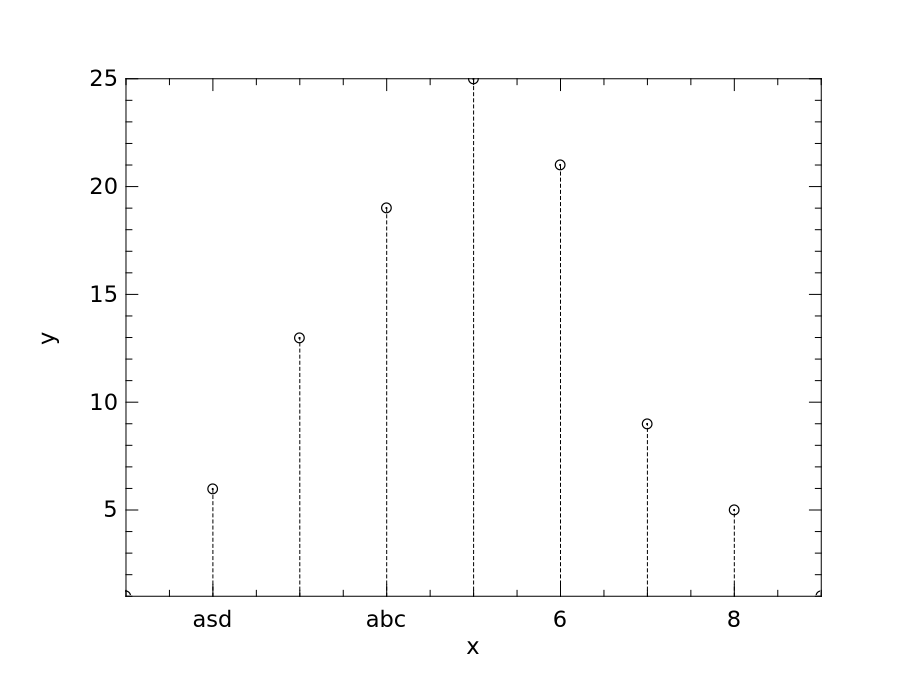
\includegraphics[width=0.4\textwidth]{figs/binompdf_hist.png} }}%
	\qquad
	\subfloat[CDF]{{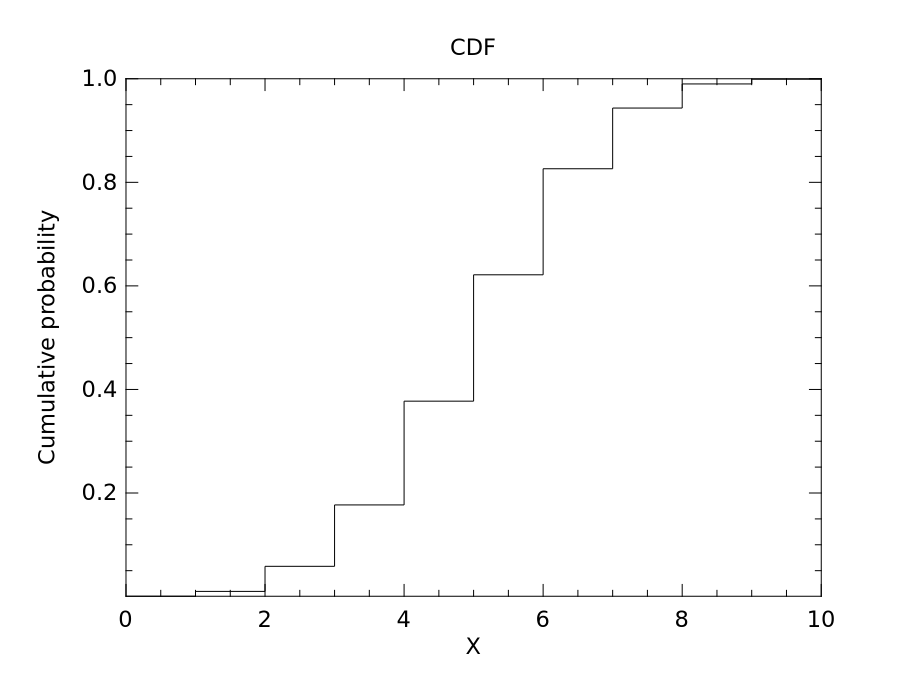
\includegraphics[width=0.4\textwidth]{figs/binom_ecdf.png} }}%
	\caption{Samples from a binomial distribution visualised, $n=10,000$}
	\label{fig:vis-binom}
\end{figure}
			
Continuous distributions are also displayed as histograms, with a set of samples being put into $n$ equal width bins. The height of each bar is the pdf, which is calculated by finding the number of samples in each bin, then dividing by the total number of samples. To display the cdf, we can display the empirical cdf directly as a scatter plot, or join points to draw a step function.
				
\begin{figure}[!htb]
	\centering
	\subfloat[PDF]{{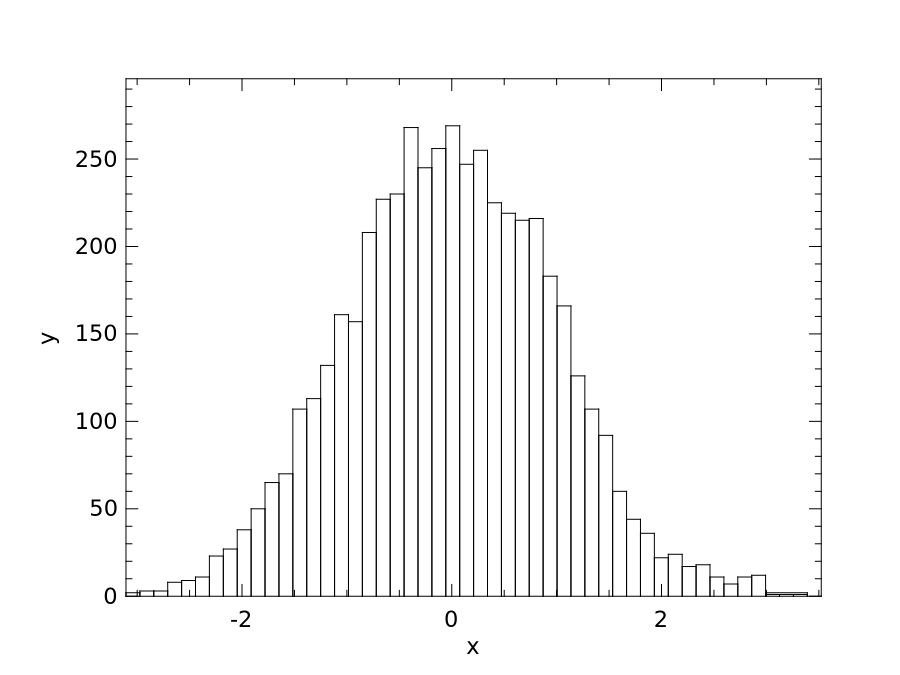
\includegraphics[width=0.4\textwidth]{figs/normpdf_hist.png} }}%
	\qquad
	\subfloat[CDF]{{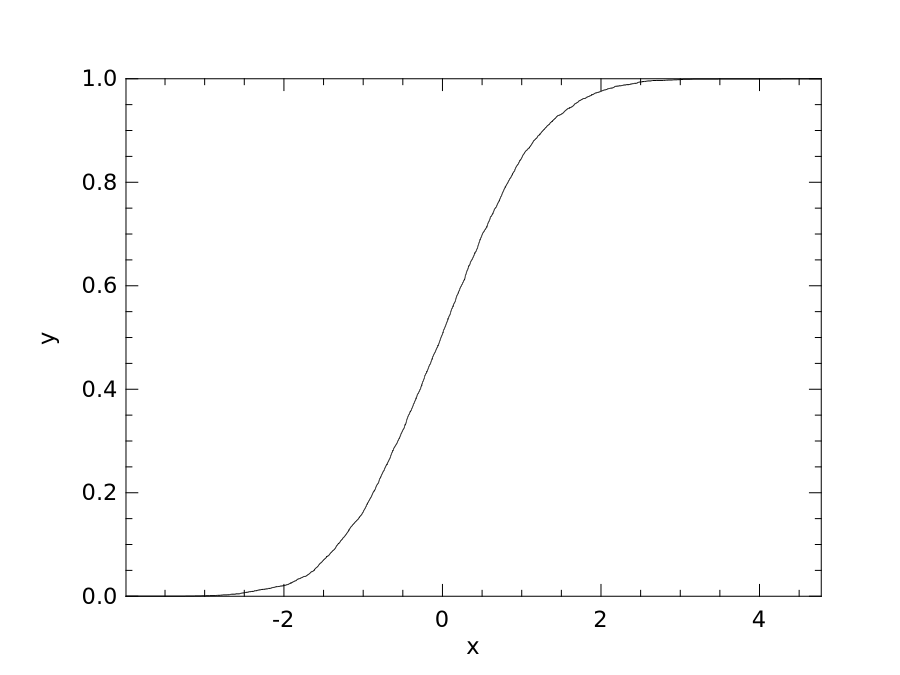
\includegraphics[width=0.4\textwidth]{figs/norm_ecdf.png} }}%
	\caption{Approximate pdf and cdf of samples from a standard normal distribution}
	\label{fig:vis-norm}
\end{figure}
				
Other important visualisations for continuous distributions are the Q-Q and P-P plots. These provides a way to qualitatively compare distributions. P-P plots plot the cdfs of two distributions against each other, that is, for two cdfs $F$ and $G$, the points $(F(z), G(z))$ are plotted for some values of z in the range $(-\infty,+\infty)$. Q-Q plots plot the quantiles of both distributions - it uses the inverse of the cdfs (the ppf) to plot the points $(F^{-1}(q), G^{-1}(q))$, where $q$, the quantile, is in the interval $[0,1]$. This plots will generally use as many points as the data allows, and calculate the percentile for every data point available. For both plots, if all the points lie on the the line $y=x$, the distributions are identical. These plots are often used to find the differences between a theoretical expected distribution and the distribution given by the data. This can be used in the PPL context to find whether a distribution given by a model matches what was expected in the theory. Figure \ref{fig:vis-qq} shows the output of inference for a model that is expected to output a beta distribution (the coin model in section \ref{sec:coin}) - the points are close to the expected line, showing successful inference.
			
\begin{figure}[!htb]
	\centering
	\subfloat[Q-Q plot]{{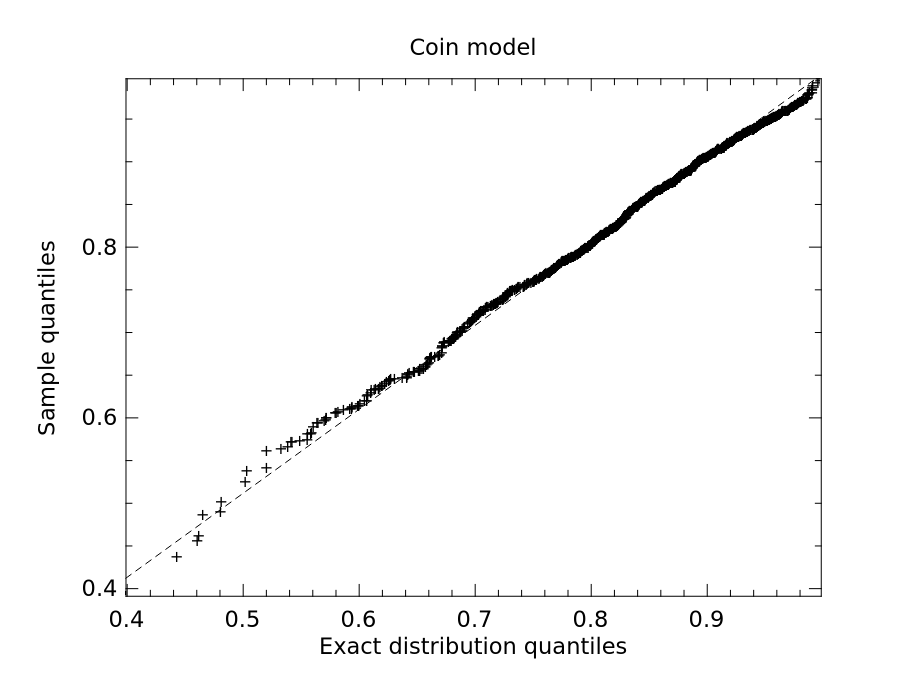
\includegraphics[width=0.4\textwidth]{figs/qq.png} }}%
	\qquad
	\subfloat[P-P plot]{{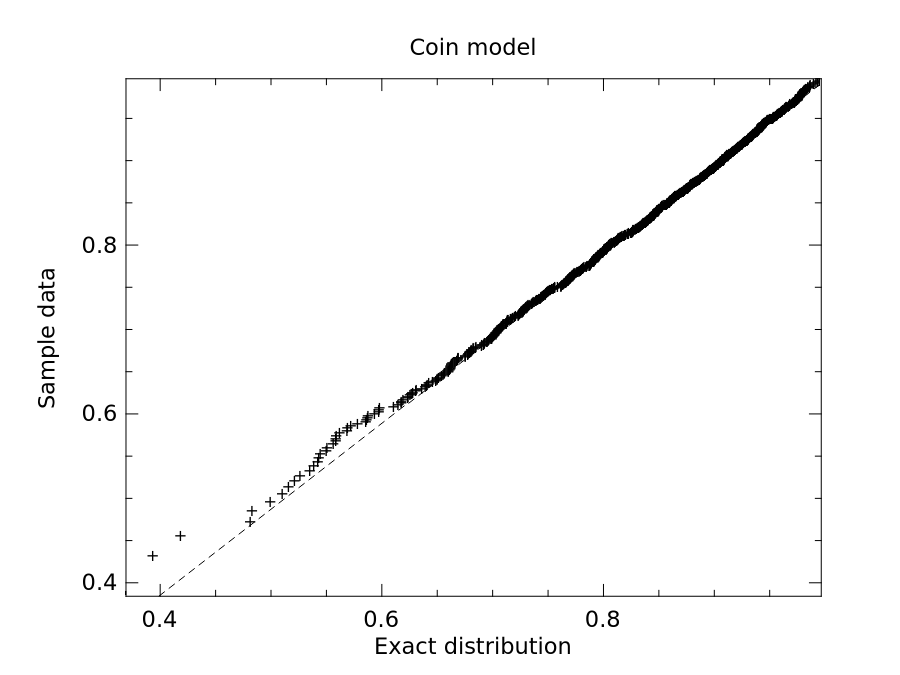
\includegraphics[width=0.4\textwidth]{figs/pp.png} }}%
	\caption{Plots to compare inferred distributions with the exact solutions}
	\label{fig:vis-qq}
\end{figure}
				
For primitive continuous distributions, a smooth line can also be drawn since we have a function that can calculate the exact pdf or cdf. This can also be overlaid onto a histogram, to compare two distributions as in figure \ref{fig:vis-samples}.
				
\begin{figure}[!htb]
	\centering														
	\begin{minipage}{0.45\textwidth}
		\centering
		\ocamlcode{code_snippets/plotter.ml}
		% \captionof{listing}{Code to produce plot}
	\end{minipage}
	\begin{minipage}{0.45\textwidth}
		\centering
		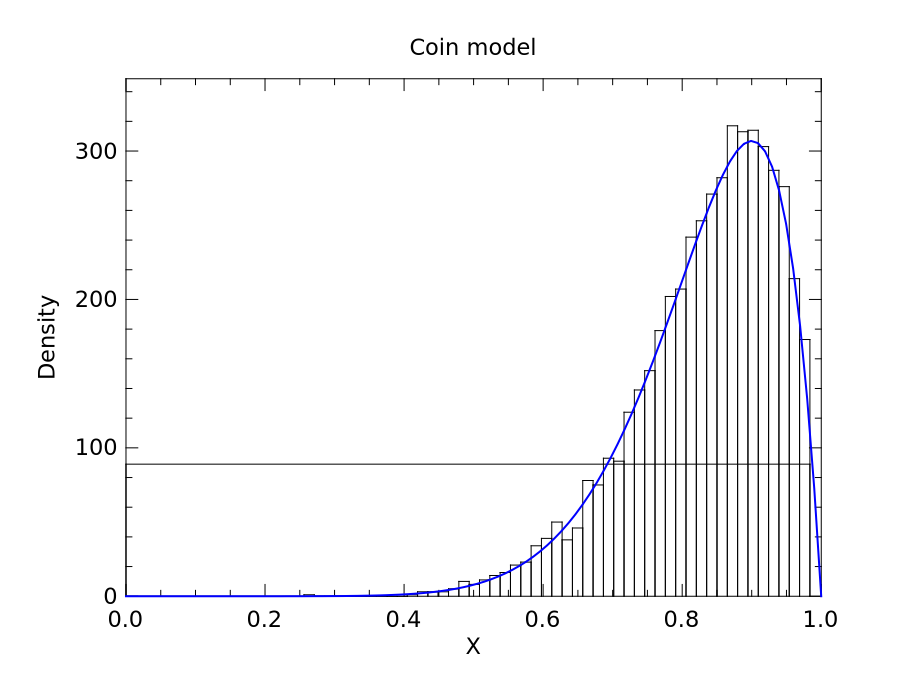
\includegraphics[width=\linewidth]{figs/coin_compare.png}
		% \captionof{figure}{Output}
	\end{minipage}
	% 
	\caption{The approximate and exact pdf of the output of inference for a biased coin model, with code to produce plot}
	\label{fig:vis-samples}
\end{figure}
				
				
\section{Testing}\label{sec:impl-testing}
			
Testing systems which are inherently random can be tricky, as it is difficult to test behaviour that is expected to change from one execution to the next. For a PPL, the most important functions to test are inference procedures, and ensuring the posterior samplers that are returned are correct. The issue is that the sequence of samples generated will change every run.
			
One approach is to set a fixed random seed and make sure the same sequence of results are produced. The aim of a unit test, however, is to make sure that a desired property does not change from one version of the code to the next. The desired property here is that the samples fit a distribution, not that the same sequence is generated. For example, for sampling from $X \sim Bernoulli(0.5)$, we might observe true,false,true,false. However, the sequence of false,true,false,true would also satisfy the distribution (and be correct), but would fail the test. Even with a fixed random seed, a change in code may cause new outputs even though the desired statistical property hasn't changed.
			
Another approach is to perform a hypothesis test such as Kolmogorov-Smirnov \cite{massey1951kolmogorov}, to ensure distributions produced by my library are equal to what is expected. The alternative hypothesis is that the samples do not fit the distribution, and we aim to not accept this. A problem with tests of this kind is that they are expected to fail sometimes. There are two possible errors:
\begin{itemize}
	\item \textit{Type 1 error} - false positive where we reject a true null hypothesis, equal to the significance level of the test.
	\item \textit{Type 2 error} - false negative where we fail to reject a false null hypothesis.
\end{itemize}
In unit testing terms, tests will sometimes fail for functions that work, and sometimes succeed for functions that are subtly broken, so unit tests based on hypothesis tests will be flaky. In fact, since we expect these tests to fail a certain percentage of the time, if they do not sometimes fail there is a problem with our program.
% maybe put the type 1/type 2 error diagram here?
			
I decided to use hypothesis testing to evaluate my PPL's inference implementations, but did not build them into automated regression testing due to their flakiness. Instead, I used weaker unit tests for inference functions, testing that they could be applied to example models and produce samples without raising any exceptions. The only inference algorithm that could be unit tested thoroughly was the exact inference method, which is deterministic and always produces the correct (exact) posterior.
			
I wrote comprehensive unit tests for the deterministic functionality. The test framework I used, \texttt{Alcotest}, checks that outputs of functions match expected values. All the helper functions (e.g. normalise), the types which could be reliably created with the same values (e.g. empirical distributions), and simple distribution properties (e.g. sampling from a Dirac distribution always produces the same value) were tested.
			
I also used an additional library \texttt{Quickcheck}, to test that a specified invariant holds for a function - it uses randomly generated inputs to check a wide range of values. As an example (listing \ref{lst:test}), for the normalise function, we expect that the output probabilities always sum to one, no matter the input array - listing \ref{lst:test}.
				
% \begin{noindent}
			\begin{listing}[!htb]
				\centering
				\begin{ocamlcode-in} 
					let test_normalise_sum_to_1 =
					QCheck.Test.make ~count:1000 ~name:"test normalisation"
					QCheck.(list (pair int float)) (* type to randomly generate *)
					(fun l -> (List.sum ~f:snd (normalise l)) = 1.)
				\end{ocamlcode-in}
				\caption{Testing the normalisation function for particles}
				\label{lst:test}
			\end{listing}
% \end{noindent}
				
A subset of the test output and code coverage are given in figure \ref{fig:test-out}.
			
\begin{figure}[!htb]
	\centering
	\subfloat[Test report, abbreviated]{{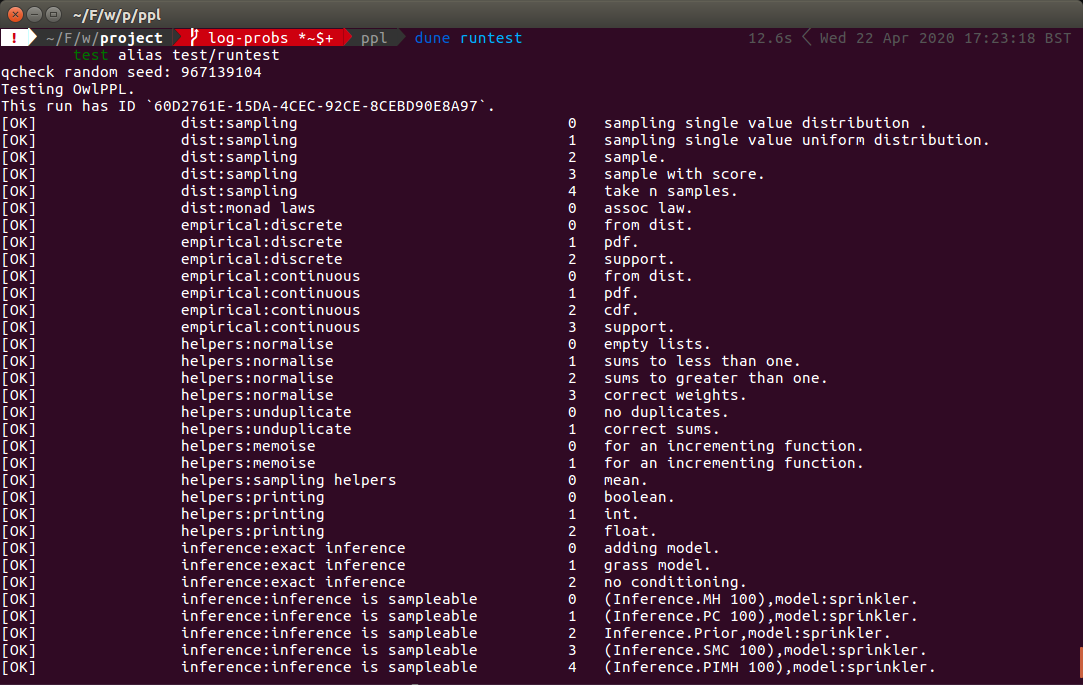
\includegraphics[width=0.6\textwidth]{figs/tests.png} }}%
	\qquad
	\subfloat[Code coverage report]{{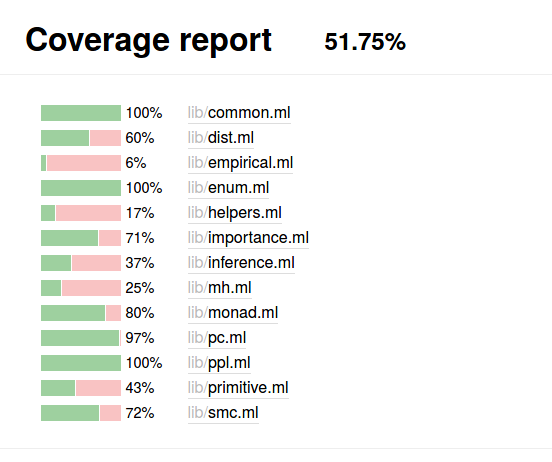
\includegraphics[width=0.35\textwidth]{figs/coverage.png} }}%
	\caption{Output from running unit tests}
	\label{fig:test-out}
\end{figure}